\documentclass[hidelinks,11pt,dvipsnames]{article}
% xcolor commonly causes option clashes, this fixes that
\PassOptionsToPackage{dvipsnames,table}{xcolor}
\usepackage[tmargin=1in, bmargin=1in, lmargin=0.8in, rmargin=1in]{geometry}

%%%%%%%%%%%%%%%%%%%%%%%%%%%%%%%%%%%%%%%%%%%%%%%%%%%%%%%%%%%%%%%%%%%%
%%% For inkscape-figures
%%% Assumes the following directory structure:
%%% master.tex
%%% figures/
%%%     figure1.pdf_tex
%%%     figure1.svg
%%%     figure1.pdf
%%%%%%%%%%%%%%%%%%%%%%%%%%%%%%%%%%%%%%%%%%%%%%%%%%%%%%%%%%%%%%%%%%%%
%\usepackage{import}
\usepackage{pdfpages}
\usepackage{transparent}

\newcommand{\incfig}[2][1]{%
    \def\svgwidth{#1\columnwidth}
    \import{./figures/}{#2.pdf_tex}
}

\pdfsuppresswarningpagegroup=1

% enable synctex for inverse search, whatever synctex is
\synctex=1
\usepackage{float,macrosabound,homework,theorem-env}
\usepackage{microtype}


% font stuff
\usepackage{sectsty}
\allsectionsfont{\sffamily}
\linespread{1.1}

% bibtex stuff
\usepackage[backend=biber,style=alphabetic,sorting=anyt]{biblatex}
\addbibresource{main.bib}

% colored text shortcuts
\newcommand{\blue}[1]{\color{MidnightBlue}{#1}}
\newcommand{\red}[1]{\textcolor{Mahogany}{#1}}
\newcommand{\green}[1]{\textcolor{ForestGreen}{#1}}


% use mathptmx pkg while using default mathcal font
\DeclareMathAlphabet{\mathcal}{OMS}{cmsy}{m}{n}

% fixes the positioning of subscripts in $$ $$
\renewcommand{\det}{\operatorname{det}}

\usetikzlibrary{positioning, arrows.meta}
\newcommand{\here}[2]{\tikz[remember picture]{\node[inner sep=0](#2){#1}}}

%%%%%%%%%%%%%%%%%%%%%%%%%%%%%%%%%%%%%%%%%%%%%%%%%%%%%%%%%%%%%%%%%%%%%
%%% Entry Counter
%%%%%%%%%%%%%%%%%%%%%%%%%%%%%%%%%%%%%%%%%%%%%%%%%%%%%%%%%%%%%%%%%%%%%
\newcounter{entry-counter}
\newcommand{\entry}[1]
{
	\addtocounter{entry-counter}{1}
    \tchap{Entry \arabic{entry-counter}}
	%\addcontentsline{toc}{section}{Entry \arabic{entry-counter}: #1}
	\vspace{-1.5em}
    \begin{center}
		\small \emph{Written: #1}
    \end{center}
}

\usepackage{titling}
\renewcommand\maketitlehooka{\null\mbox{}\vfill}
\renewcommand\maketitlehookd{\vfill\null}


\usepackage{capt-of}
\usepackage{tikz}
\usepackage{listings}
\usetikzlibrary{positioning,calc,intersections,through,backgrounds, shapes.geometric, decorations.markings,arrows}

\def\sset{\subseteq}
\def\iso{\cong}
\def\gend#1{\langle #1\rangle}

\newcommand{\rightoverleftarrow}{%
  \mathrel{\vcenter{\mathsurround0pt
    \ialign{##\crcr
      \noalign{\nointerlineskip}$\longrightarrow$\crcr
      \noalign{\nointerlineskip}$\longleftarrow$\crcr
    }%
  }}%
}

\newcommand\makesphere{} % just for safety
\def\makesphere(#1)(#2)[#3][#4]{%
  % Synopsis
  % \makesphere[draw options](center)(initial angle:final angle:radius)
  \shade[ball color = #3, opacity = #4] #1 circle (#2);
  \draw #1 circle (#2);
  \draw ($#1 - (#2, 0)$) arc (180:360:#2 and 3*#2/10);
  \draw[dashed] ($#1 + (#2, 0)$) arc (0:180:#2 and 3*#2/10);
}
% same thing as makesphere but places white background behind
\newcommand\altmakesphere{} % just for safety
\def\altmakesphere(#1)(#2)(#3)[#4][#5]{%
  % Synopsis
  % \make sphere[draw options](center)(initial angle:final angle:radius)
  \draw [fill=white!30] #1 circle (#2);
  \shade[ball color = #4, opacity = #5] #1 circle (#2);
  \draw #1 circle (#2);
  \draw ($#1 - (#2, 0)$) arc (180:360:#2 and 3*#2/10);
  \draw[dashed] ($#1 + (#2, 0)$) arc (0:180:#2 and 3*#2/10);
  \node at #1 {#3};
}

\begin{document}
% set section number to 1
% fixes theorem numbering without need to have a section title
\setcounter{section}{1}

\pagestyle{empty}
	\LARGE
\begin{center}
	Foundations of Data Science and Machine Learning -- \emph{Homework 5}\\
	\Large
	Isaac Martin \\
    Last compiled \today
\end{center}
\normalsize
\vspace{-4mm}
\hru

\begin{homework}[e]
  \prob Suppose $\bfA$ is a $n\times d$ full-rank matrix, with $n < d$, and fix $\bfb\in \bR^n$. Consider minimizing the least squares objective $F(\bfx) = \|\bfA\bfx - \bfb\|^2_2$ Note that in this setting, the solution space $\cS = \{x : \bfA\bfx = \bfb\}$ is an affine subspace of $\bR^d$. We use gradient descent with constant step-size:
  \begin{align*}
    \bfx = \bfx_{k-1} - \eta \nabla F(\bfx_{k-1}).
  \end{align*}
  \begin{enumerate}[(a)]
    \item Give an upper bound for the step-size $\eta$ such that gradient descent is guaranteed to converge for $\eta$ below this threshold.
    \item Suppose that gradient descent is initialized at $\bfx_0 = 0$. Show that when gradient descent converges, it must converge to the least-norm solution $\bfx^* = \operatorname{argmin}_{\bfx \in \cS} \|\bfx\|^2_2$.
  \end{enumerate}
  \begin{prf}$ $
    \begin{enumerate}[(a)]
      \item In class, we showed that if $\nabla F$ is Lipschitz with Lipschitz constant $L$, then choosing $\eta = 1/L$ guarantees the convergence of gradient descent. In particular, any $\eta \leq 1/L$ will guarantee the convergence of gradient descent, so we need only find $L$. We have
        \begin{align*}
        \|\nabla F(\bfx) - \nabla F(\bfy)\|_2 
          &= \|2\bfA^\top(\bfA \bfx - \bfb) - 2\bfA^\top(\bfA \bfy - \bfb)\|_2 \\
          &= \|2\bfA^\top \bfA(\bfx - \bfy)\|_2 \\
          &\leq 2\|\bfA^\top \bfA\|\cdot \|\bfx - \bfy\|_2
        \end{align*}
        where $\|\cdot\|$ denotes the operator norm. Hence choosing $\eta \leq (2\|\bfA^\top\bfA\|)^{-1}$ will guarantee the convergence of gradient descent for any initialization.

      \item Let us first prove the hint, namely, that if $\bfx \in \img\bfA^\top$ (i.e. if $\bfx$ is in the rowspan of $\bfA$) then so is $A\bfx - \eta \nabla F(\bfx)$. Suppose then that $\bfx = \bfA^\top \bfu$ for some $\bfu \in \bR^n$. Then
        \begin{align*}
          \bfy = \bfA \cdot \bfA^\top \bfu - \nabla F(\bfA^\top \bfu) 
            &=\bfA \cdot \bfA^\top \bfu - \nabla 2A^\top(\bfA \bfA^\top \bfu - \bfu) \\
            &= \bfA^\top u - 2\eta \bfA^\top \bfA \bfA^\top \bfu - 2\bfA^\top \bfb \\
            &= \bfA^\top\left(\bfu - 2\eta \bfA\bfA^\top \bfu - 2\bfb\right) \implies \bfy \in \img \bfA^\top.
        \end{align*}
        Because the update rule is continuous and the image of affine linear transformations is closed, we can further conclude that an initialization $\bfx_0$ is in the rowspan of $\bfA$ if and only if the point $\bfx^*$ it converges to is in the rowspan of $\bfA$, provided $\eta$ is chosen small enough to guarantee convergence.

        \bigskip

        Now we prove that any two points initialized in the rowspan of $\bfA$ converge to the same point. Take $\bfx_0 = \bfA^\top \bfu_0$ to be an initialization for some $\bfu_0 \in \bR^n$. By what we have previously shown, $\bfx^* = \bfA^\top \bfu^*$ for some $\bfu^* \in \bR^n$, supposing we have chosen $\eta$ to be small enough. Since $\bfx^*$ is a stable point of the update rule, we get that $\nabla F(\bfx^*) = 0$ and hence
        \begin{align*}
          \nabla F(\bfA^\top \bfu^*) = 2\bfA^\top(\bfA\bfA^\top &\bfu^* - \bfb) = 0 \\
            &\implies \bfA^\top(\bfA\bfA^\top \bfu^* - \bfb) = 0\\
            &\implies \bfA^\top \bfu^* - \bfb = 0
        \end{align*}
        since $\bfA$ is full rank with $n < d$ (so $\ker A^\top = 0$). This means $\bfu^* = (\bfA\bfA^\top)^{-1}\bfb$, noting that the inverse $(\bfA\bfA^\top)^{-1}$ exists again because $\bfA$ is fully rank with $n < d$. Using this expression for $\bfu^*$ gives us that $\bfx^* = \bfA^\top(\bfA\bfA^\top)^{-1}\bfb$, which notably does not depend on the initialization, implying that any two points initialized in the rowspan of $\bfA$ converge to the same point.

        \bigskip

        Finally, consider two different initialization $\bfy_0 \in \bR^d \setminus \img(A^\top)$ and $\bfx_0 \in \img(A^\top)$. As before, $\bfx_0 = \bfA^\top \bfu$ for some $\bfu \in \bR^n$. Since $\bfy_0$ is not in the rowspan of $\bfA$, the stable point $\bfy^*$ of the update rule to which $\bfy_0$ converges is also not in $\img(\bfA^\top)$. Hence $\bfy^* = \bfA^\top \bfu^* + \bfv$ for some $\bfv \not\in \img\bfA^\top$, where $\bfu^*$ is as above. The stability condition $\nabla F(\bfy^*) = 0$ gives us $\bfA\bfA^\top \bfu^* + \bfA\bfv - \bfb = 0$ repeating the calculation from the last paragraph. But $\bfA\bfA^\top \bfu^* - \bfb = 0$, so $\bfA\bfv = 0$. This means
        \begin{align*}
          \|\bfy^*\|^2_2 
            &= (\bfA^\top \bfu^* + \bfv)^\top (\bfA^\top \bfu^* + \bfv) \\
            &= \bfu^\top \bfA^\top \bfA \bfu + \bfu^\top \bfA v + (\bfA\bfv)^\top \bfu + \bfv^\top \bfv \\
            &= \bfu^\top \bfA^\top \bfA \bfu + 0 + 0 + \bfv^\top \bfv \\
            &\geq \bfu^\top \bfA^\top \bfA \bfu \\
            &= \|\bfx^*\|^2_2.
        \end{align*}
        Thus, $\bfx^* = \arg\min_{\bfx\in \cS} \|\bfx\|^2_2$. Any point in the rowspan of $\bfA$ converges to $\bfx^*$ under the update rule; in particular, the initialization $\bfx_0 = 0$ converges to $\bfx^*$, proving the desired result.
    \end{enumerate}
  \end{prf}

  \prob Let $f:\bR^d \to \bR$ be a differentiable function. It satisfies the PL-inequality if there exists a constant $\mu > 0$ such that for all $w \in \bR^d$ it holds
  \begin{align*}
    \frac{1}{2}\|\nabla f(w)\|^2_2 \geq \mu(f(w) - f^*).
  \end{align*}
  By contrast we say $f$ is \emph{invex} if there exists a function $\eta:\bR^d\times \bR^d\to \bR^d$ such that for all $x, y\in \bR^d$ it holds
  \begin{align*}
    f(y) \geq f(x) + \nabla f(x)^\top \eta(x,y).
  \end{align*}
  \begin{enumerate}[(a)]
    \item Show that if $f$ satisfies the PL-inequality then $f$ is invex.
    \item Show that any stationary point of an invex function is a global minimizer.
  \end{enumerate}
  \begin{prf}$ $
    \begin{enumerate}[(a)]
      \item Since $f$ satisfies the PL-inequality, for some $\mu > 0$
        \begin{align*} 
          \frac{1}{2}\|\nabla f(w)\|^2_2 \geq \mu(f(w) - f^*)
        \end{align*}
        for all $w\in \bR^d$, where $f^*$ is the global minimum of $f$. Rearranging, we get
        \begin{align*}
          &\hspace{5em}\frac{1}{2}\|\nabla f(w)\|^2_2 \geq \mu(f(w) - f^*) \\
            &\implies \nabla f(w)^\top \nabla f(w) \geq 2\mu f(w) - 2\mu f^* \\
            &\implies - \nabla f(w)^\top \nabla f(w) \leq 2\mu f^* - 2\mu f(w) \leq f(w) \leq 2\mu f(u) - 2\mu f(w)
        \end{align*}
        for any $w, u\in \bR^d$, since $f^*$ is the global minimum of $f$. This in turn implies that
        \begin{align*}
          2\mu f(w) - \nabla f(w)^\top \nabla f(w) \leq 2\mu f(u),
        \end{align*}
        so if we set $\eta(x,y) = - \frac{1}{2\mu}\nabla f(x)$ then we get
        \begin{align*}
          f(x) = \nabla f(x)^\top \cdot \eta(x,y) \leq f(y)
        \end{align*}
        for all $x, y\in \bR^d$. This proves that $f$ is invex.

      \item A point $\bfx$ is a stationary point of $f$ if $\nabla f(x) = 0$. If $f$ is invex, then we get
        \begin{align*}
          f(y) \geq f(x) + \nabla f(x)^top \eta(x,y) = f(x)
        \end{align*}
        for all $y\in \bR^d$. Hence any stationary point of $f$ is a global minima. Combining with part (a) we see that any function which satisfies the PL-inequality is easily optimized.
    \end{enumerate}
  \end{prf}
  \prob In your favorite programming language, implement stochastic gradient-descent for the linear least squares loss $f(\bfw) = \frac{1}{2}\|\bfA\bfW - \bfb\|^2_2$. Provide convergence plots to validate the convergence guarantees for SGD discussed in class. Specifically, compare empirical and theoretical convergence rates when $\bfA \in \bR^{10,000\times 1,000}$ has iid $\cN(0, 1/\sqrt{1000})$ Gaussian entries and $\bfb = \bfA\mathbf{1} + \epsilon$ where $\mathbf{1}$ is the all-ones vector and $\epsilon$ has iid Gaussian antries with variance 1, then 0.1, then 0.01 and finally 0. Repeat the comparisons but now consider $\bfA \in \bR^{10000 \times 1000}$ whose $j$th row has iid $\cN(0,1/\sqrt{1000j})$ Gaussian entries. (\emph{Note your answer should include 8-plots, because there are two choices of $\bfA$ and four different choices of $\epsilon$.})
  \begin{prf} $ $
    Here is the first round of graphs with $A$ chosen to be a $10^4 \times 10^3$ matrix with entries normally sampled from $\cN(0,1/\sqrt{10000})$, denoted by $A_1$ below. The batchsize was chosen to be 100, and sgd was allowed to run for 100 iterations with a step size of 0.1. The theoretical bound is shown in red and the empirical result in blue.
    \begin{center}
      \centering
      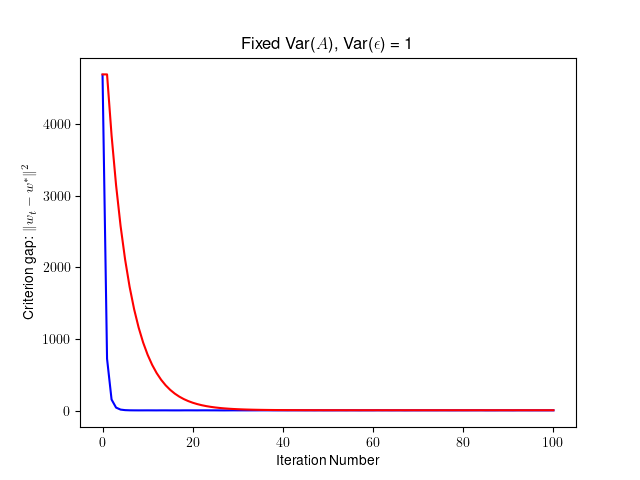
\includegraphics[width=0.45\textwidth]{figures/graph1.png}
      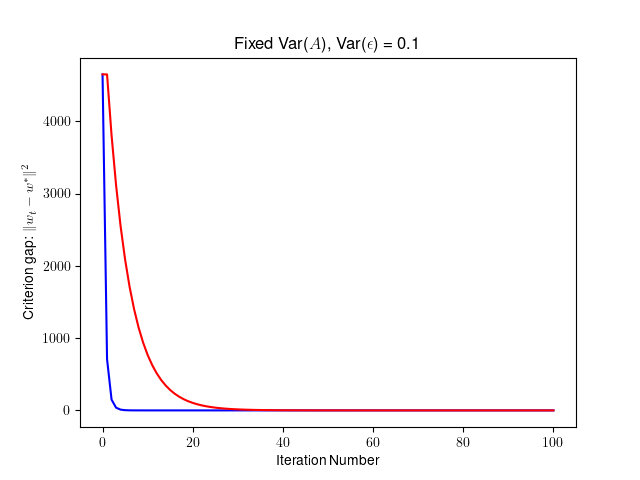
\includegraphics[width=0.45\textwidth]{figures/graph2.png}

      \bigskip

      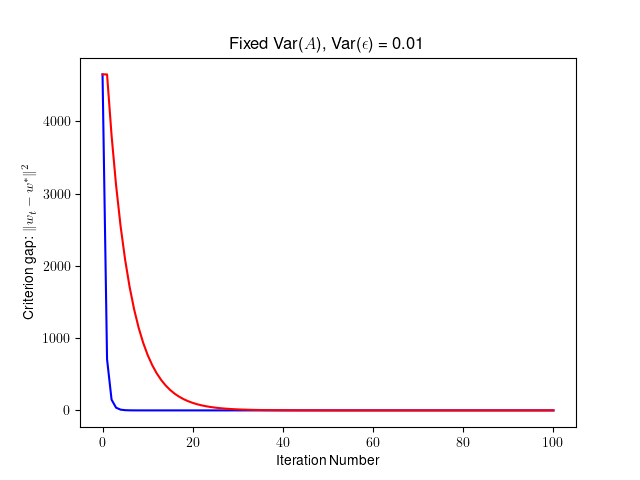
\includegraphics[width=0.45\textwidth]{figures/graph3.png}
      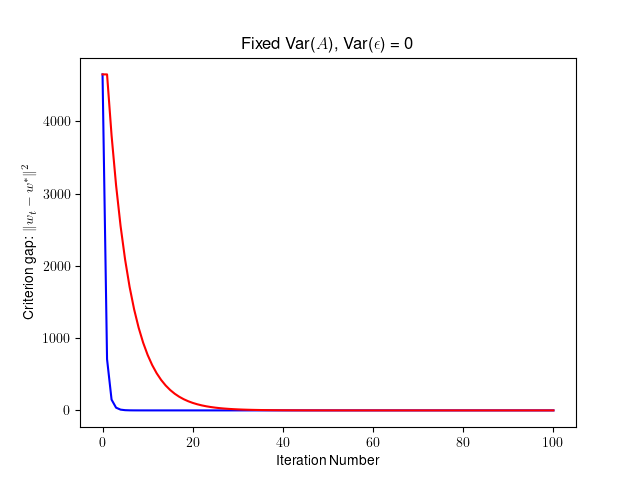
\includegraphics[width=0.45\textwidth]{figures/graph4.png}
      \captionof{figure}{First round of images, theoretical bound in red and empirical result in blue.}
    \end{center}
    Here is the second round of plots where $A$ was chosen to be a $10^4\times 10^3$ matrix whose $j$th row had entries sampled from $\cN(0,1/\sqrt{10000j})$, denoted by $A_2$ below. The batchsize was chosen to be 10, and as the convergence was slower, the algorithm was allowed to run for 1000 iterations with a step size of 0.1.
    \begin{center}
      \centering
      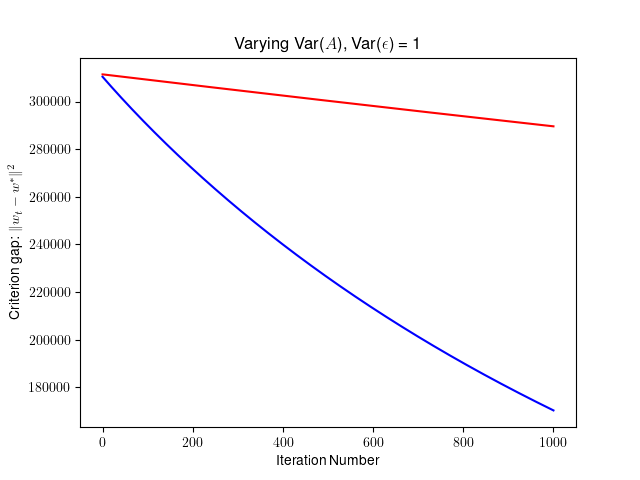
\includegraphics[width=0.45\textwidth]{figures/graph5.png}
      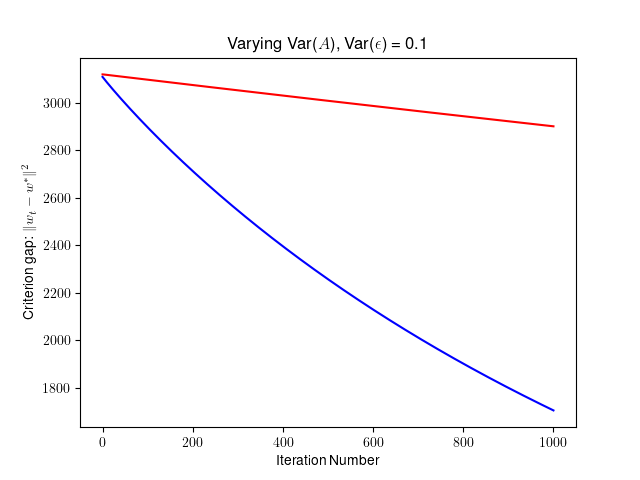
\includegraphics[width=0.45\textwidth]{figures/graph6.png}

      \bigskip

      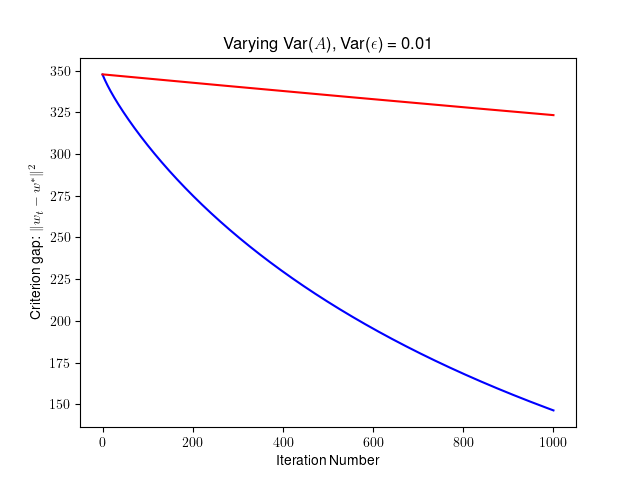
\includegraphics[width=0.45\textwidth]{figures/graph7.png}
      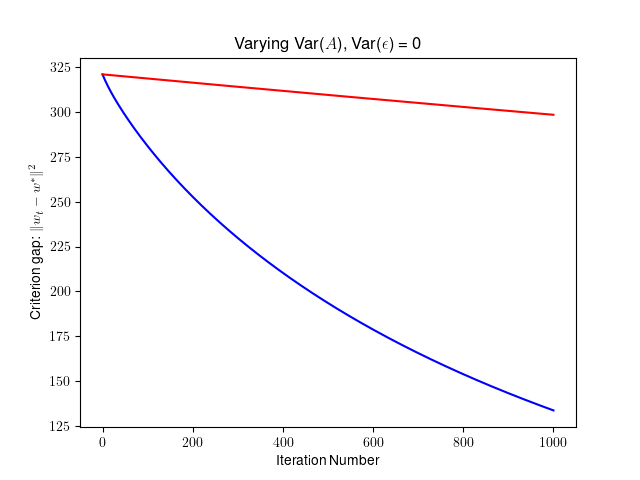
\includegraphics[width=0.45\textwidth]{figures/graph8.png}
      \captionof{figure}{Second round of images, theoretical bound in red and empirical result in blue.}
    \end{center}
    The theoretical result was pretty good in the first round of plots, but it was shockingly loose in the second round. I'm not sure why this is, and to be honest, I don't fully trust my implementation of it. The bound used was the following, taken from Slide 16 of Lecture 18:
    \begin{align*}
      \bE\|w_t - w_*\|^2_2 \leq (1 - 2\alpha \mu(1 - \alpha L))^t \|w_0 - w_*\|^2_2 + \alpha \frac{\sigma^2}{\mu(1 - \alpha L)},
    \end{align*}
    where
    \begin{itemize}
      \item $\mu = \lambda_{min}(A^\top A)$
      \item $L = n\cdot \max_j \|a_j\|^2_2$ where $a_j$ is the $j$th row of $A$
      \item $\sigma^2 =\frac{1}{n}\sum_{j=1}^n \|\nabla f_j(w_*)\|^2 $
      \item $\alpha$ is the stepsize, reset to $1/2L$ if larger than $1/L$.
    \end{itemize}
    I did make one change to this bound, I multiplied $t$ in the exponent by the batchsize. This sped up the convergence, but may not be theoretically correct in general.

    Here is a table presenting the results in another way. I believe the error would have continued to fall for the $A_2$ case, if more iterations were used. I wasn't patient enough to let it run for longer, however.
    \begin{center}  
      \begin{tabular}{cc|ccc|ccc}
        & & & Experimental &&& Theoretical & \\
        $A$ & $\nu^2$ & Initial Error & Final Error & Reduction \% & Initial Error & Final Error & Reduction \\
        \hline
            $A_1$ & 1 & 4690.1205 & 4.6306 & 99.9013 & 4696.5921 & 6.4717 & 99.8622 \\
            $A_1$ & 0.1 & 4647.4501 & 0.0477 & 99.9990 & 4647.5172 & 0.0669 & 99.9985 \\
            $A_1$ & 0.01 & 4651.7212 & 0.0004672 & 99.9999 & 4651.7219 & 0.0006495 & 99.9999 \\
            $A_1$ & 0 & 4651.9180 & 1.5432e-09 & 99.9999 & 4651.9180 & 1.1542 & 99.9999 \\
        \hline
        $A_2$ & 1 & 310402.7632 & 170335.4203 & 45.1243 & 311385.3539 & 289588.1955 & 7.0000 \\
        $A_2$ & 1 & 3108.1134 & 1705.7998 & 45.1178 & 3118.6050 & 2900.3430 & 6.9986 \\
        $A_2$ & 1 & 347.6325 & 146.3506 & 57.9008 & 347.7354 & 323.3239 & 7.0201 \\
        $A_2$ & 1 & 321.1256 & 133.5297 & 58.4182 & 321.1256 & 298.5754 & 7.0222\\
        \hline
      \end{tabular}
    \end{center}
  \end{prf}
  \prob Consider a three-state Markov chain with stationary probabilities $\left(\frac{1}{2}, \frac{1}{3},\frac{1}{6}\right)$. consider the Metropolis-Hastings algorithm with $G$ the complete graph on these three vertices. For each edge and each direction, what is the expected probability that we would actually make a move along the edge?
  \begin{prf}
    Recall that the Metropolis transition probabilities are
    \begin{align*}
      p_{xy} = \frac{1}{r}\min \left(1, \frac{\pi(y)}{\pi(x)}\right) 
    \end{align*}
    if $x$ and $y$ are distinct but adjacent and
    \begin{align*}
      p_{xx} = 1 - \sum_{y\neq x} p_{xy}.
    \end{align*}
    Let $a,b$ and $c$ be the vertices of the graph. Then
    \begin{align*}
      p_{ab} &= \frac{1}{2}\frac{2}{1}\cdot \frac{1}{3} = \frac{1}{3} \\
      p_{ac} &= \frac{1}{2}\frac{2}{1}\cdot \frac{1}{6} = \frac{1}{6} \\
      p_{aa} &= 1 - \frac{1}{3} - \frac{1}{6} = \frac{1}{2}.
    \end{align*}
    The other transition probabilities are
    \begin{align*}
      p_{ba} = \frac{1}{2}, \hspace{1.5em} p_{bc} = \frac{1}{4}, \hspace{1.5em} p_{bb} = \frac{1}{4}
    \end{align*}
    and
    \begin{align*}
      p_{ca} = \frac{1}{2}, \hspace{1.5em} p_{cb} = \frac{1}{2}, \hspace{1.5em} p_{cc} = 0.
    \end{align*}
  \end{prf}
  \prob Consider the probability distribution $p(\bfx)$ where $\bfx \in \{0,1\}^{100}$ such that $p(0) = \frac{1}{2}$ and $p(\bfx) = \frac{1/2}{2^{100}-1}$. How does Gibbs sampling behave here?
  \begin{prf}
    The Gibbs transition probabilities are given by
    \begin{align*}
      p_{xy} =
      \begin{cases}
        \frac{1}{d}\pi(y_i ~|~ x_1,...,\hatx_i,...,x_d) & \text{ if $\bfx$ and $\bfy$ differ only in $i$} \\
        0 & \text{ otherwise }
      \end{cases}.
    \end{align*}
    Let $\hate_i$ denote the element of $\{0,1\}^{100}$ whose $i$th component is 1 and is 0 elsewhere.
    We have three cases to examine.

    \bigskip 

    \noindent\emph{If we are currently at }$\mathbf{0}$, then
    \begin{itemize}
    \item there is a $\frac{1}{100}\frac{\frac{1/2}{2^{100}-1}}{\frac{1}{2}+\frac{1/2}{2^{100}-1}} \approx \frac{1}{100}\cdot \frac{1}{2^{100}-1}$ chance of moving to $\hate_i$ for any $i \in \{1,...,100\}$. Altogether, we have a $1$ in $2^{100} - 1$ chance of leaving $0$ at all.
    \item We have a $1 - \frac{1}{2^{100}-1}\approx 1$ chance of remaining at zero.
    \end{itemize}
    Hence, if we ever reach 0 then we will stay at zero, since $2^{100}-1$ is a huge number.

    \bigskip

    \noindent\emph{If we are currently at }$\hate_i$, then we
    \begin{itemize}
      \item have a $\frac{1}{100}\frac{1/2}{\frac{1}{2}+\frac{1/2}{2^{100}-1}}\approx \frac{1}{100}$ chance of moving to 0.
      \item have a $\frac{1}{100}\frac{\frac{1/2}{2^{100}-1}}{\frac{1/2}{2^{100}-1} + \frac{1/2}{2^{100}-1}}\approx \frac{1}{200}$ chance of moving to some other nonzero point, of which there are 99 adjacent to $\hate_i$ giving us an approximately $\frac{1}{2}$ chance point of moving to a point which is not $0$
      \item have an approximately $1 - \frac{1}{100} - \frac{1}{2} = \frac{1}{2}-\frac{1}{100}$ chance of remaining at $\hate_i$.
    \end{itemize}

    \bigskip

    \emph{If we are currently at } $\bfx\neq \hate_i, \mathbf{0}$, then we
    \begin{itemize}
      \item have a $\frac{1}{100}\frac{\frac{1/2}{2^{100}-1}}{\frac{1/2}{2^{100}-1}+\frac{1/2}{2^{100}-1}} \approx \frac{1}{200}$ chance of moving to any individual neighbor of $\bfx$, or altogether a $1$ in $2$ chance of leaving $\bfx$ to \emph{some} other point
      \item have an $1 - 100\cdot \frac{1}{200} \approx \frac{1}{2}$ chance of remaining at $\bfx$.
    \end{itemize}

    If we initialize a random walk on $G$ at $\mathbf{0}$ then we will remain there functionally forever. If we initialize it at any other point, then we have a $\frac{1}{2}$ chance to leave and a $\frac{1}{2}$ chance to remain. The situation is slightly different at a point neighboring $\mathbf{0}$, where we have twice the chance of transitioning to $\mathbf{0}$ than to any other point. Thus, a random walk on $G$ will visit a variety of points, transitioning to a new point every $2$ steps on average, unless it reaches $\mathbf{0}$, in which case it will remain there indefinitely. However, the chance of reaching $\mathbf{0}$ from a random initialization is just as small as the chance of leaving $\mathbf{0}$, since there are $2^{100}$ points in total.
  \end{prf}
  \prob Let $\bfA \in \bR^{m\times n}$ be a matrix with rank exactly $k$. Consider the following randomized procedure:
  \begin{itemize}
    \item Draw a matrix $\bfG \in \bR^{n\times k}$ with i.i.d. $\cN(0,1)$ Gaussian entries.
    \item Form the matrix $\bfY = \bfA\bfG \in \bR^{m\times k}$.
    \item Form the matrix $\bfZ = \bfA^\top \bfY \in \bR^{n\times k}$
  \end{itemize}
  Is it possible to reconstruct $\bfA$ and its singular value decomposition from the information provided by the matrices $(\bfG, \bfY, \bfZ)$? If yes, then specify and algorithm. If no, then provide a counterexample.
  \begin{prf}
    The answer is 'yes'. Perhaps this expected, for we know that $\bfG$ has full rank $k$. Indeed, because of this, and because if $B$ has full rank then $\rank (AB) = \rank (A)$, we know that $\bfY = \bfA\bfG$ has rank $k$. This means $\bfY$ has reduced SVD
    \begin{align*}
      \bfY = U_Y \Sigma_Y V^\top_Y.
    \end{align*}
    Because $\bfY$ is $m\times k$ and is rank $k$, it is full rank and hence $\bfZ = \bfA^\top\bfY$ has rank $k$. Thus $\bfZ$ has reduced SVD $U_Z\Sigma_ZV^\top_Z$, giving us
    \begin{align*}
      \bfZ = U_Z\Sigma_ZV^\top_Z = \bfA^\top \bfY = \bfA^\top U_Y \Sigma_Y V^\top_Y.
    \end{align*}
    As $\bfY$ is of full rank $k$, we may find a matrix $M$ such that $A^\top \bfY C = A^\bfY$ (hand waving has occurred). Solving for $\bfA^\top$ using this fact gives us
    \begin{align*}
      A^T &= U_Z\Sigma_Z V_Z(U_Y\Sigma_Y V_Y^\top)^\top C \\
        &= U_Z\Sigma_Z V_Z^\top V_Z \Sigma_Y U_Y^\top C \\
        &= U_Z \Sigma_Z\Sigma_Y U_Y^\top C
    \end{align*}
    Notice that this is an SVD, $\Sigma_Z\Sigma_Y$ is diagonal. Hence we can recover the SVD of $\bfA$ (and hence $\bfA$) by calculating the SVD of $\bfY$ and $\bfZ$ and setting $U_A = C^\top U_Y$, $\Sigma_A = \Sigma_Y\Sigma_Z$ and $V_A = U_Z$.
  \end{prf}
\end{homework}
\newpage
\begin{verbatim}  
  from multiprocessing import Value
  from matplotlib.pyplot import plot
  import numpy as np
  import math
  from sklearn.datasets import fetch_california_housing
  from sklearn.model_selection import train_test_split


  def sgd(
      gradient,
      gradient_js,
      x,
      y,
      start,
      ideal,
      learn_rate=0.1,
      batch_size=1,
      n_iter=50,
      tolerance=1e-06,
      dtype="float64",
      random_state=None,
      plot_title="",
      mul=1,
      filename="",
  ):
      # Checking if the gradient is callable
      if not callable(gradient):
          raise TypeError("'gradient' must be callable")

      # Setting up the data type for NumPy arrays
      dtype_ = np.dtype(dtype)

      # Converting x and y to NumPy arrays
      x, y = np.array(x, dtype=dtype_), np.array(y, dtype=dtype_)
      n_obs = x.shape[0]
      if n_obs != y.shape[0]:
          raise ValueError("'x' and 'y' lengths do not match")
      # Make matrix out of all x and y points, smash the matrices together columnwise
      # This makes shuffling easier later on by shuffling x and y simultaneously
      xy = np.c_[x.reshape(n_obs, -1), y.reshape(n_obs, 1)]

      # Initializing the random number generator
      seed = None if random_state is None else int(random_state)
      rng = np.random.default_rng(seed=seed)

      # Initializing the values of the variables
      vector = np.array(start, dtype=dtype_)

      # Setting up and checking the learning rate
      learn_rate = np.array(learn_rate, dtype=dtype_)
      if np.any(learn_rate <= 0):
          raise ValueError("'learn_rate' must be greater than zero")

      # Setting up and checking the size of minibatches
      batch_size = int(batch_size)
      print("batch_size:", batch_size)
      if not 0 < batch_size <= n_obs:
          raise ValueError(
              "'batch_size' must be greater than zero and less than "
              "or equal to the number of observations"
          )

      # Setting up and checking the maximal number of iterations
      n_iter = int(n_iter)
      if n_iter <= 0:
          raise ValueError("'n_tier' must be greater than zero")

      # Setting up and checking the tolerance
      tolerance = np.array(tolerance, dtype=dtype_)
      if np.any(tolerance <= 0):
          raise ValueError("'tolerance' must be greater than zero")

      # initialize plotting variables
      accuracy = []
      theoretical = []
      iter_num = []

      # deriving constants
      # lecture 18 page 16
      def terms_in_bound(learn_rate):
          # get eigenvalues, n, and all norms of the rows of x
          eig, _ = np.linalg.eig(np.matmul(x.T, x))
          n = x.shape[0]
          row_norm = [(np.linalg.norm(x[j, :])) ** 2 for j in range(rows)]

          # get sigma
          inp_diff = [np.abs((np.dot(x[j, :], ideal) - y[j])) ** 2 for j in range(n)]
          sigma2 = (
              n ** (1.4)
              * sum([row_norm[j] * inp_diff[j] for j in range(n)])
              / (batch_size**2)
          )[0]

          # get the constants L, mu, alpha etc
          mu = min(sorted(eig))
          L = n * max(row_norm)

          if learn_rate >= 1 / (L):
              alpha = 1 / (2 * L)

          else:
              alpha = learn_rate
          grad = gradient(x, y, ideal)

          print("alpha: ", alpha)
          print("L: ", L)
          print("mu: ", mu)
          print("sigma^2: ", sigma2)

          # terms in bound
          coeff = 1 - 2 * alpha * mu * (1 - alpha * L)
          norm = np.linalg.norm(start - ideal) ** 2
          frac = alpha * (sigma2) / (mu * (1 - alpha * L))
          print(f"alpha: {alpha}\nalpha/(mu(1 - alpha*L)): {frac/sigma2}")
          return coeff, norm, frac

      def theory_bound(i, coeff, norm, frac):
          return (coeff**i) * norm + frac

      # compute these terms once
      coeff, norm, frac = 0, 0, 0
      if plot_title:
          coeff, norm, frac = terms_in_bound(learn_rate=learn_rate)
          print(coeff, norm, frac)

      accuracy.append(np.linalg.norm(start - ideal) ** 2)
      theoretical.append(theory_bound(0, coeff, norm, frac))
      iter_num.append(0)
      # Performing the gradient descent loop
      for i in range(n_iter):
          # Shuffle x and y
          rng.shuffle(xy)

          # Performing minibatch moves
          for start in range(0, n_obs, batch_size):
              stop = start + batch_size
              x_batch, y_batch = xy[start:stop, :-1], xy[start:stop, -1:]

              # Recalculating the difference
              grad = np.array(gradient(x_batch, y_batch, vector), dtype_)
              diff = -learn_rate * grad
              # Checking if the absolute difference is small enough
              if np.all(np.linalg.norm(diff) <= tolerance):
                  break

              # Updating the values of the variables
              vector += diff

          acc = np.linalg.norm(vector - ideal) ** 2
          # print(f"completed iteration {i}, ||pred - b|| = {acc}")
          if plot_title:
              iter_num.append(i + 1)
              accuracy.append(acc)
              theoretical.append(theory_bound(i * mul, coeff, norm, frac))

      if plot_title:
          import matplotlib.pyplot as plt

          plt.rcParams.update({"text.usetex": True, "font.family": "Helvetica"})
          plt.plot(iter_num, accuracy, c="b")
          plt.plot(iter_num, theoretical, c="r")
          plt.xlabel("Iteration Number")
          plt.ylabel(r"Criterion gap: $ \|w_t- w^*\|^2 $")
          plt.title(plot_title)
          plt.savefig(filename)
          plt.close()

      print("\n\nExperimental, Theoretical")
      print(
          accuracy[0],
          "&",
          accuracy[-1],
          "&",
          ((accuracy[0] - accuracy[-1]) / accuracy[0]) * 100,
          "&",
          theoretical[0],
          "&",
          theoretical[-1],
          "&",
          ((theoretical[0] - theoretical[-1]) / theoretical[0]) * 100,
      )
      print("\n")
      return vector if vector.shape else vector.item()


  # the rows and columns of the matrices in this problem
  rows = 10000
  cols = 1000

  # the various epsilons
  ep1 = np.random.normal(0, 1, size=(rows, 1))
  ep2 = np.random.normal(0, 0.1, size=(rows, 1))
  ep3 = np.random.normal(0, 0.01, size=(rows, 1))
  ep4 = np.random.normal(0, 0, size=(rows, 1))

  # a cols x 1 column vector, correct shape to multiply with A
  ones = np.ones(shape=(cols, 1))


  def problem3a():
      mu = 0
      sigma = 1 / math.sqrt(cols)
      A = np.random.normal(mu, sigma, (rows, cols))

      # setup the b and w vectors
      M = np.matmul(np.linalg.inv(np.matmul(np.transpose(A), A)), np.transpose(A))
      b0 = np.matmul(A, ones)
      bs = [b0 + ep1, b0 + ep2, b0 + ep3, b0 + ep4]
      w_min = [np.matmul(M, b) for b in bs]
      w_0 = np.random.uniform(low=0, high=5, size=(cols, 1))

      # hyper-parameters
      stepsize = 0.1
      batch_size = 100
      num_iter = 100
      mul = 1000

      # graphing
      titles = [
          r"Fixed Var($A$), Var($\epsilon$) = 1",
          r"Fixed Var($A$), Var($\epsilon$) = 0.1",
          r"Fixed Var($A$), Var($\epsilon$) = 0.01",
          r"Fixed Var($A$), Var($\epsilon$) = 0",
      ]
      filenames = ["graph1.png", "graph2.png", "graph3.png", "graph4.png"]

      def grad_loss(X, y, w):
          """
          Gradient of the least squares loss function
          """
          return np.matmul(np.transpose(X), np.matmul(X, w) - y)

      def grad_loss_js(X, y, w):
          """
          Gradient of the least squares loss function for the jth part
          """
          AtA = np.matmul(X.transpose(), X)
          n = w.shape[0]
          stupid = [AtA[:, j].reshape((n, 1)) * w[j] for j in range(n)]
          Atb = np.matmul(X.transpose(), y)
          print(AtA)
          print(Atb)
          print()

          components = [stupid[j] + (Atb / n) for j in range(n)]
          return components

      for i in range(len(bs)):
          b = bs[i]
          w_best = w_min[i]
          title = titles[i]
          sgd(
              gradient=grad_loss,
              gradient_js=grad_loss_js,
              x=A,
              y=bs[i],
              start=w_0,
              learn_rate=stepsize,
              ideal=w_min[i],
              batch_size=batch_size,
              n_iter=num_iter,
              plot_title=titles[i],
              mul=mul,
              filename=filenames[i],
          )


  def problem3b():
      mu = 0
      sigma = lambda j: 1 / math.sqrt(cols * j)
      A = np.array([np.random.normal(mu, sigma(j), (cols)) for j in range(1, rows + 1)])

      # setup the b and w vectors
      M = np.matmul(np.linalg.inv(np.matmul(np.transpose(A), A)), np.transpose(A))
      b0 = np.matmul(A, ones)
      bs = [b0 + ep1, b0 + ep2, b0 + ep3, b0 + ep4]
      w_min = [np.matmul(M, b) for b in bs]
      w_0 = np.random.uniform(0, 1, size=(cols, 1))

      # hyper-parameters
      stepsize = 0.1
      batch_size = 10
      num_iter = 1000
      mul = 1000

      # graphing
      titles = [
          r"Varying Var($A$), Var($\epsilon$) = 1",
          r"Varying Var($A$), Var($\epsilon$) = 0.1",
          r"Varying Var($A$), Var($\epsilon$) = 0.01",
          r"Varying Var($A$), Var($\epsilon$) = 0",
      ]
      filenames = ["graph5.png", "graph6.png", "graph7.png", "graph8.png"]

      def grad_loss(X, y, w):
          """
          Gradient of the least squares loss function
          """
          return np.matmul(np.transpose(X), np.matmul(X, w) - y)

      def grad_loss_js(X, y, w):
          """
          Gradient of the least squares loss function for the jth part
          """
          AtA = np.matmul(X.transpose(), X)
          n = w.shape[0]
          stupid = [AtA[:, j].reshape((n, 1)) * w[j] for j in range(n)]
          Atb = np.matmul(X.transpose(), y)
          print(AtA)
          print(Atb)
          print()

          components = [stupid[j] + (Atb / n) for j in range(n)]
          return components

      for i in range(len(bs)):
          b = bs[i]
          w_best = w_min[i]
          title = titles[i]
          sgd(
              gradient=grad_loss,
              gradient_js=grad_loss_js,
              x=A,
              y=bs[i],
              start=w_0,
              learn_rate=stepsize,
              ideal=w_min[i],
              batch_size=batch_size,
              n_iter=num_iter,
              plot_title=titles[i],
              mul=mul,
              filename=filenames[i],
          )


  problem3b()
\end{verbatim}
\end{document}
